
\documentclass[17pt]{beamer}

\usepackage{graphicx}
\usepackage{array}
\usepackage{xspace}
\usepackage{xcolor}
\usepackage{bbm}
\usepackage{soul}

\usepackage{tikz}
\usetikzlibrary{positioning}


\setbeamercolor{title}{fg=red}
\setbeamercolor{frametitle}{fg=red}
\setbeamercolor{section in head/foot}{bg=red}
\setbeamercolor{author in head/foot}{bg=red}
\setbeamercolor{date in head/foot}{fg=red}

\newcommand{\nat}{\ensuremath{\mathbb N}\xspace}
\newcommand{\nphard}{{{\np}-hard}\xspace}
\newcommand{\sharpP}{\ensuremath{\#\mathbf{P}}\xspace}
\newcommand{\set}[1]{\left\{#1\right\}}
\newcommand{\floor}[1]{\left\lfloor{#1}\right\rfloor}
\newcommand{\pr}[1]{\left(#1\right)}
\newcommand{\fpr}[1]{\mathopen{}\left(#1\right)}
\newcommand{\spr}[1]{\left[#1\right]}
\newcommand{\fspr}[1]{\mathopen{}\left[#1\right]}
\newcommand{\brak}[1]{\left<#1\right>}
\newcommand{\abs}[1]{{\left|#1\right|}}
\newcommand{\norm}[1]{\left\|#1\right\|}
\newcommand{\enset}[2]{\left\{#1 ,\ldots , #2\right\}}
\newcommand{\enpr}[2]{\pr{#1 ,\ldots , #2}}
\newcommand{\enlst}[2]{{#1} ,\ldots , {#2}}
\newcommand{\vect}[1]{\spr{#1}}
\newcommand{\envec}[2]{\vect{#1 ,\ldots , #2}}
\newcommand{\real}{\mathbb{R}}
\newcommand{\np}{\textbf{NP}\xspace}
\newcommand{\naturals}{\mathbb{N}}
\newcommand{\funcdef}[3]{{#1}:{#2} \to {#3}}
\newcommand{\define}{\leftarrow}
\newcommand{\reals}{{\mathbb{R}}\xspace}
\newcommand{\proba}[1]{\text{Pr}\left({#1}\right)\xspace}
\newcommand{\bigO}{\ensuremath{\mathcal{O}}\xspace}

\newcommand{\txtred}[1]{\textcolor{red}{#1}}
\newcommand{\txtgreen}[1]{\textcolor{green!70!black}{#1}}
\newcommand{\txtgray}[1]{\textcolor{gray}{#1}}
\renewcommand{\hl}[1]{\textcolor{magenta}{#1}}
\newcommand{\ind}[1]{\ensuremath{\mathbbm{1}\spr{#1}}}

\newcommand{\ruleset}{\ensuremath{S}}
\newcommand{\crule}{\ensuremath{R}}
\newcommand{\data}{\ensuremath{D}}
\newcommand{\posdata}{\ensuremath{\data_{+}}}
\newcommand{\negdata}{\ensuremath{\data_{-}}}

\newcommand{\poisson}{\ensuremath{\text{Poisson}}}

\newcommand{\minposthresh}{\ensuremath{\tau_{+}}}
\newcommand{\maxnegthresh}{\ensuremath{\tau_{-}}}

\newcommand{\expt}{\ensuremath{\mathop{\mathbb{E}}}}

\newcommand{\sectionslide}[1]{ 
  \begin{frame}  
    \vfill
    \begin{center}   
      {\LARGE \txtred{#1}}  
    \end{center}
    \vfill
  \end{frame}
}

\tikzset{% 
}
  

\title{Lunar New Year}
\date{\today}



\begin{document}

\frame{\titlepage}

\sectionslide{What?}

\begin{frame}
  \frametitle{Lunar New year}

  \begin{itemize}
  \item also know as \txtred{Chinese New Year} or \txtred{Spring New Year}
  \item the most important festival for the Chinese
  \end{itemize}
\end{frame}

\sectionslide{When?}

\begin{frame}
  \frametitle{}

  \begin{itemize}
  \item marks the start of \txtgreen{spring} and \txtred{the next lunar year}
  \item usually between late Jan. and early Feb. (solar calendar)
  \item usually lasts $\sim$ 1 week
  \end{itemize}
\end{frame}

\sectionslide{Why? the origin}

\begin{frame}
  \frametitle{the ``Nian'' beast (Nian hirviö)}

  \begin{center}
    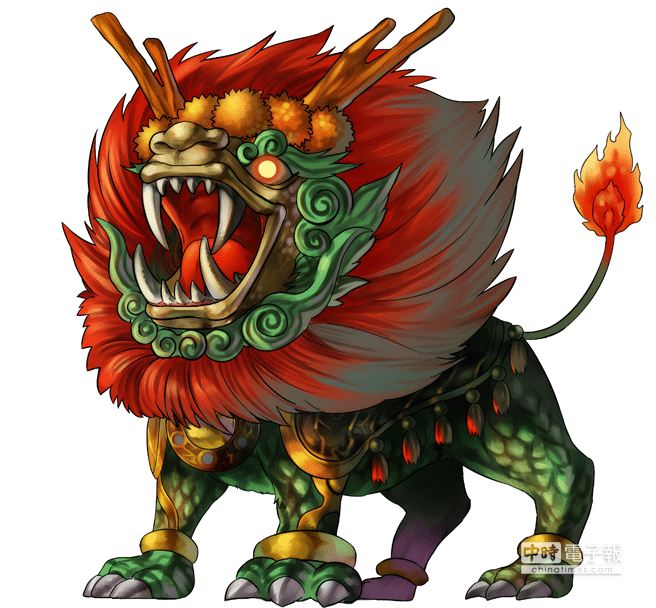
\includegraphics[width=0.8\textwidth]{./images/nian}
  \end{center}
\end{frame}

\begin{frame}
  \frametitle{what Nian fears}

\begin{itemize}
\item loud sound
\item red color
\item flashing light
\end{itemize}
\end{frame}

\begin{frame}
  \frametitle{the red lantern (punaiset lyhty)}

  \begin{center}
    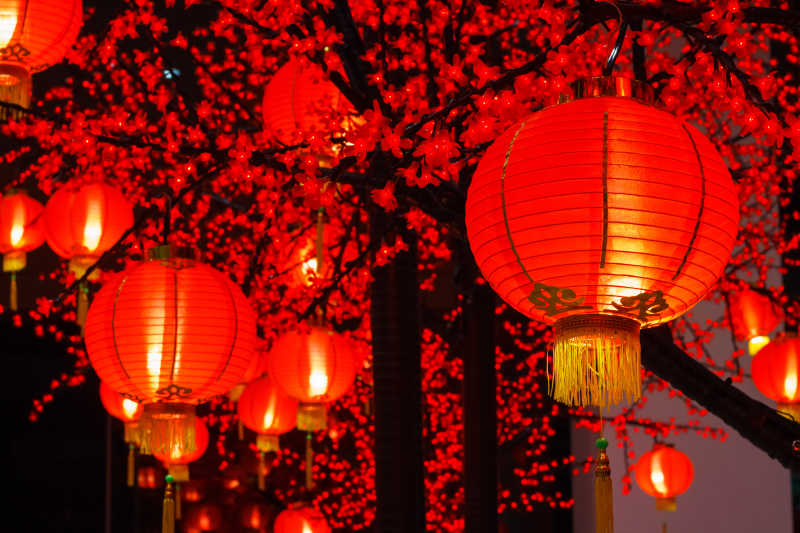
\includegraphics[width=0.8\textwidth]{./images/red-lantern}
  \end{center}
\end{frame}

\begin{frame}
  \frametitle{fire crackers (sähinkäiset)}
  \begin{center}
    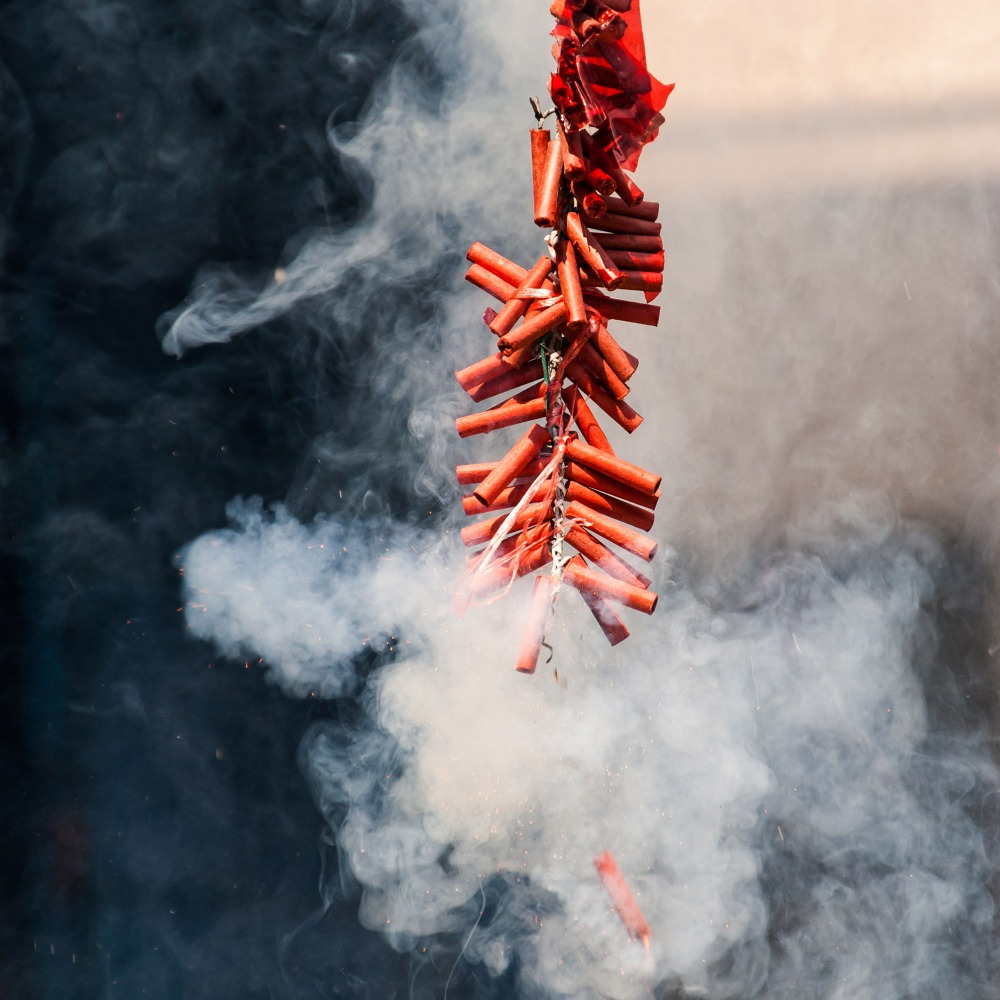
\includegraphics[width=.7\textwidth]{./images/firework1}
  \end{center}
\end{frame}


\begin{frame}
  \frametitle{spring festival scroll (kupletit)}
  \begin{center}
    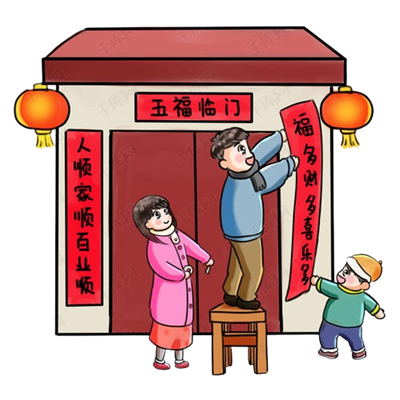
\includegraphics[width=.7\textwidth]{./images/chunlian}
  \end{center}
\end{frame}

\begin{frame}
  \frametitle{paper cut for window (ikkunan paperileikkaus)}
  \begin{center}
    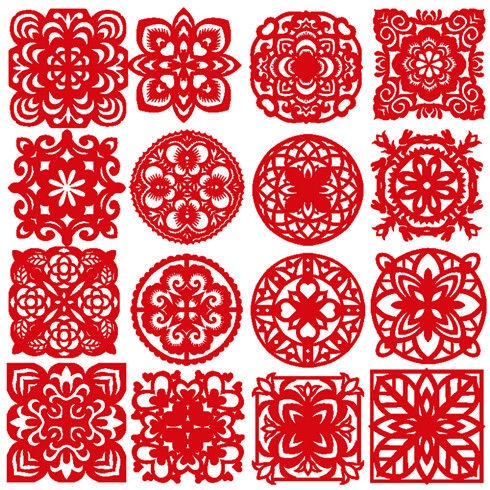
\includegraphics[width=.6\textwidth]{./images/chuanghua1}
  \end{center}
\end{frame}

\sectionslide{How? what do we do}

\begin{frame}
  \frametitle{family time}

  \begin{center}
    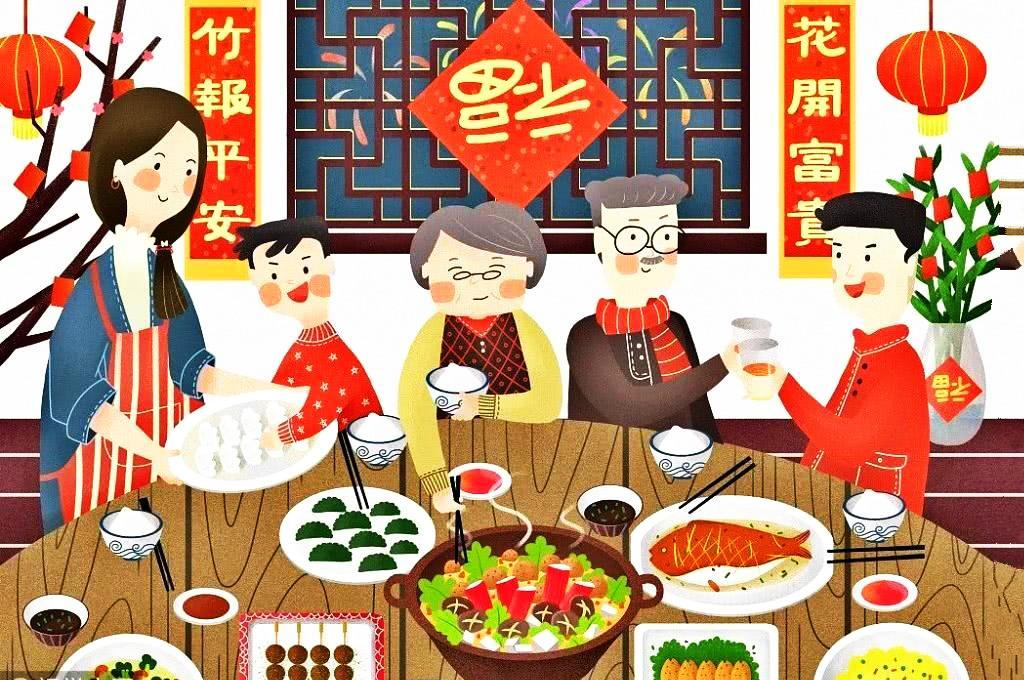
\includegraphics[width=0.8\textwidth]{./images/tuanju}
  \end{center}
\end{frame}

\begin{frame}
  \frametitle{new year greetings}
  \begin{center}
    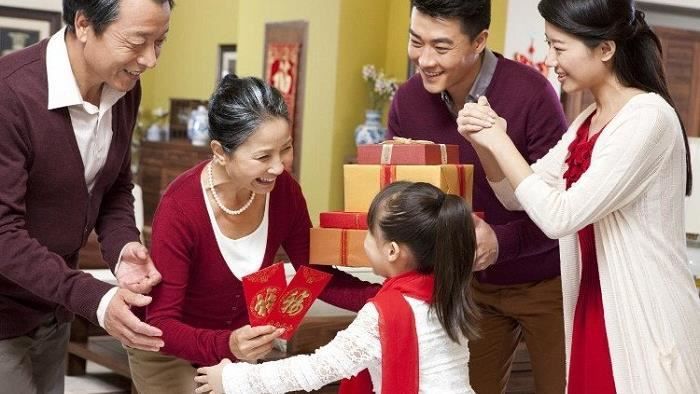
\includegraphics[width=.9\textwidth]{./images/bainian}
  \end{center}
\end{frame}

\begin{frame}
  \frametitle{the red envelope (punaiset kirjekuori)}
  \begin{center}
    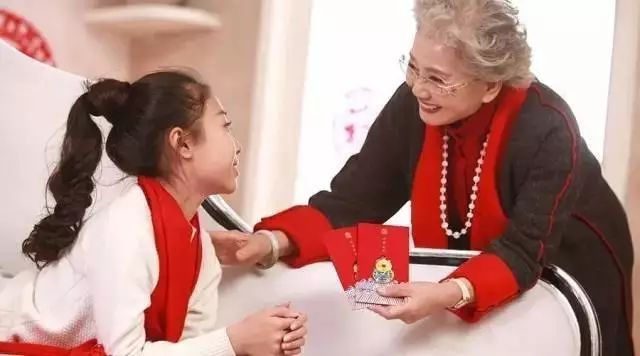
\includegraphics[height=.35\textheight]{./images/hongbao}\quad
    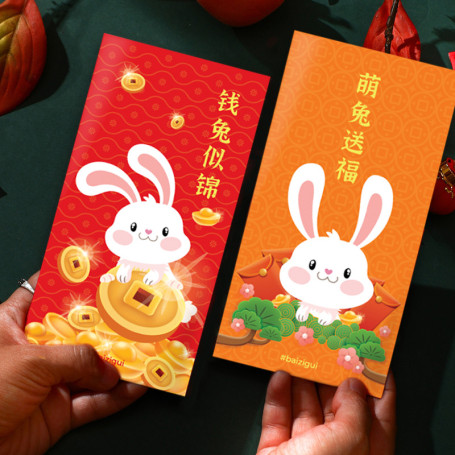
\includegraphics[height=.35\textheight]{./images/hongbao1}
  \end{center}  
\end{frame}

\begin{frame}
  \frametitle{temple fair (temppelijuhla)}
  \begin{center}
    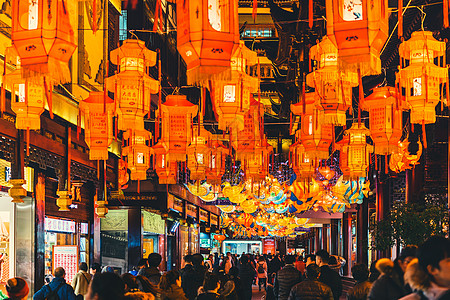
\includegraphics[height=.75\textheight]{./images/miaohui}
  \end{center}    
\end{frame}

\begin{frame}
  \frametitle{\visible<2>{lion} dance}
  \begin{center}
    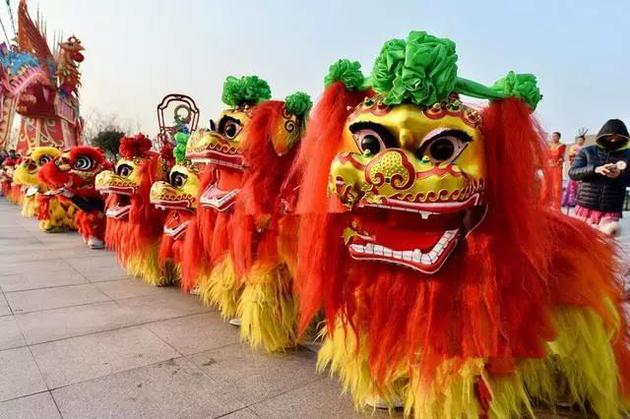
\includegraphics[height=.75\textheight]{./images/wushi}
  \end{center}
\end{frame}

\begin{frame}
  \frametitle{dragon dance}
  \begin{center}
    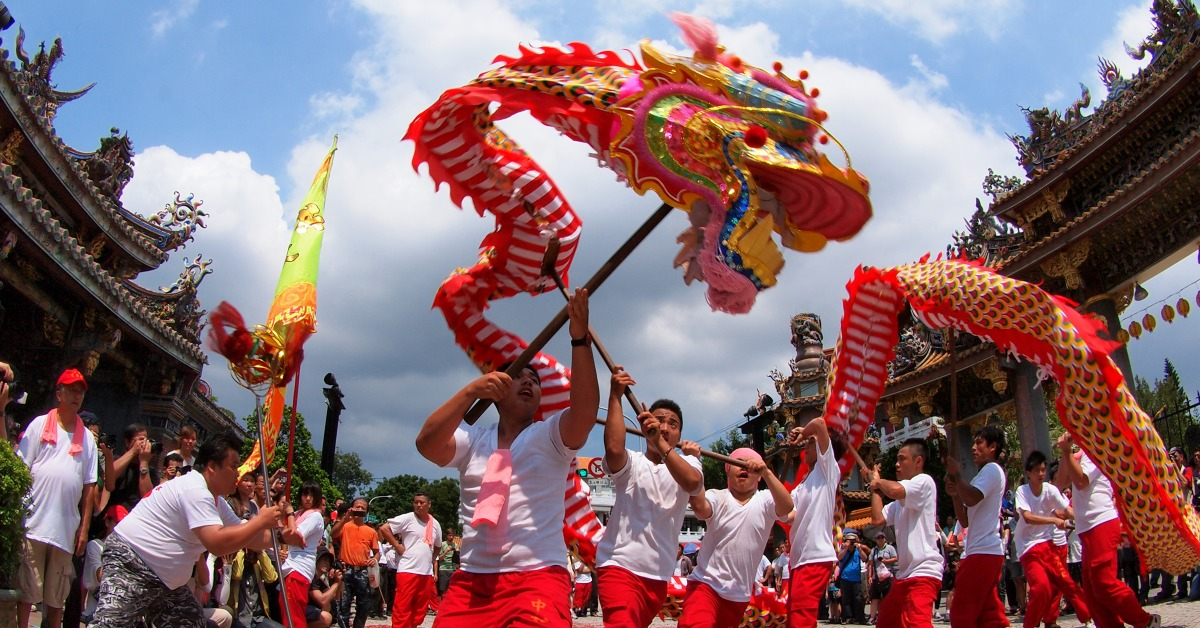
\includegraphics[height=.6\textheight]{./images/wulong}
  \end{center}
\end{frame}

\sectionslide{Food?}

\begin{frame}
  \frametitle{dumplings}
  \begin{center}
    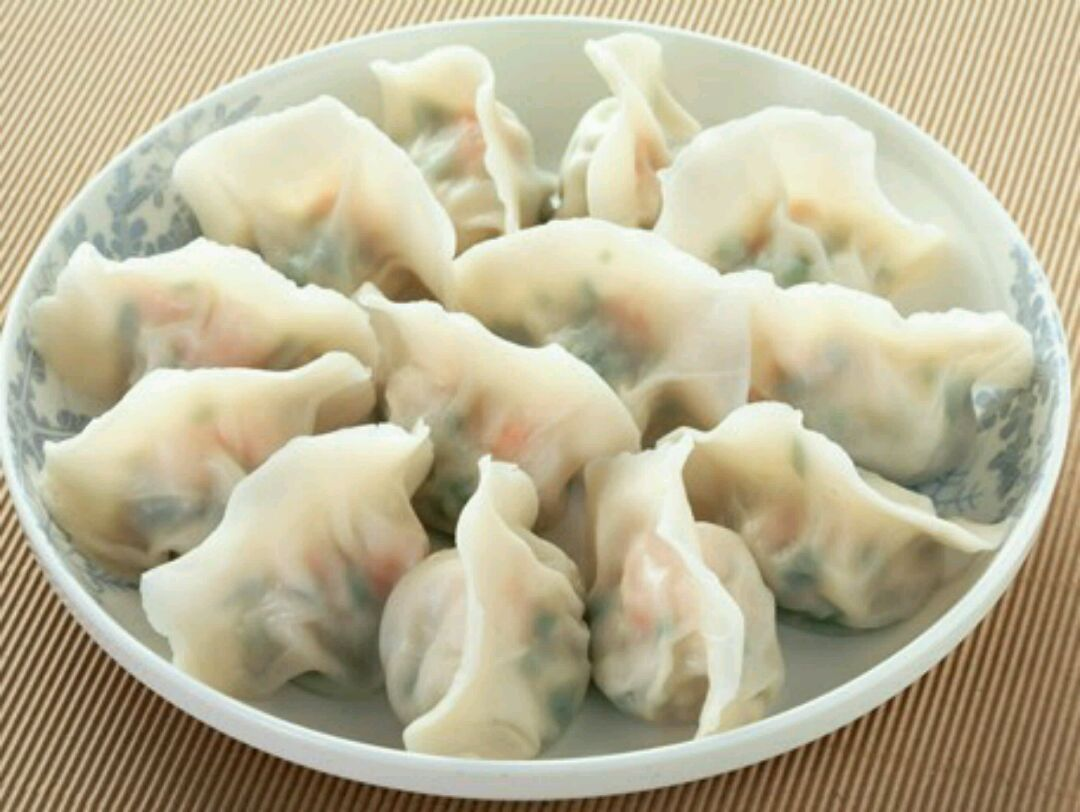
\includegraphics[height=.6\textheight]{./images/jiaozi}
  \end{center}  
\end{frame}

\begin{frame}
  \frametitle{candied haws (orapihlaja)}
    \begin{center}
    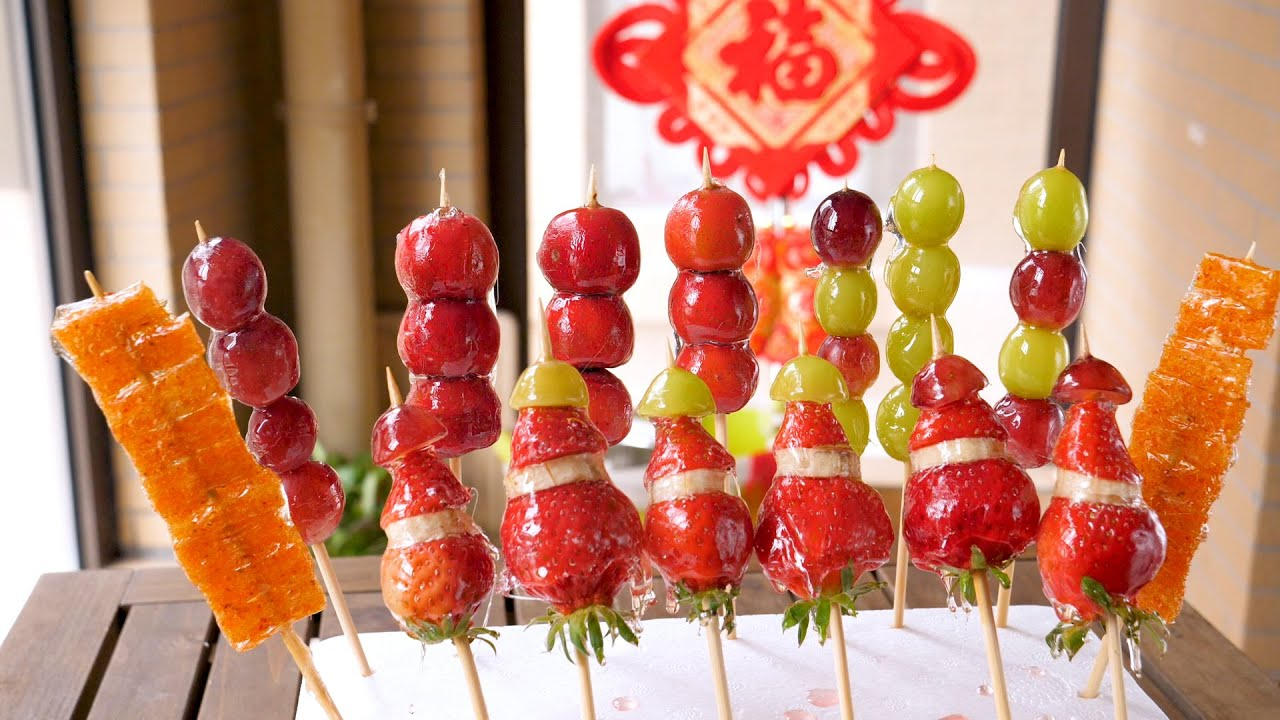
\includegraphics[height=.6\textheight]{./images/tanghulu}
  \end{center}
\end{frame}

\begin{frame}
  \frametitle{sticky rice dumplings}
      \begin{center}
    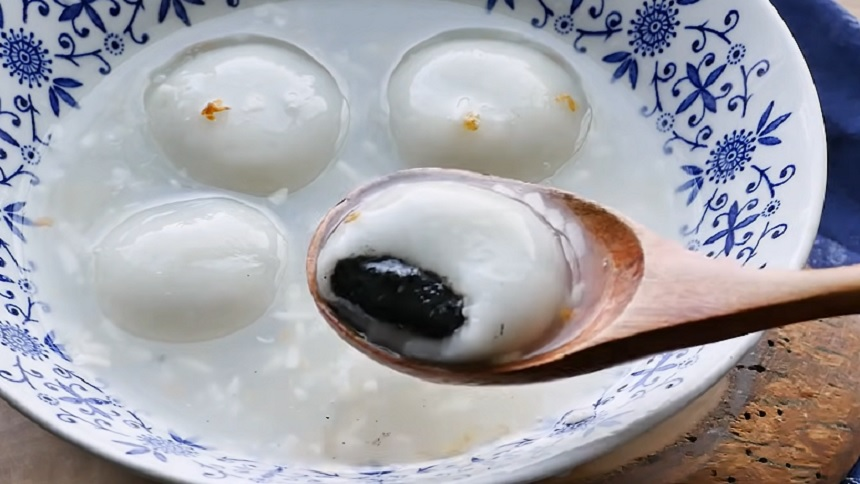
\includegraphics[height=.6\textheight]{./images/tangyuan}
  \end{center}
\end{frame}
\end{document}
